%!TEX root = ../main.tex

\chapter{Marco tecnológico}\label{cap:marco-tecnologico}

\section{Vista en capas}

La arquitectura de la plataforma se estructura en cuatro capas principales, presentación, lógica de negocio y API, datos, y servicios externos. Este esquema modular facilita el desarrollo, la realización de pruebas y el escalado de cada componente de forma independiente, optimizando los tiempos de trabajo cuando el proyecto está a cargo de un único desarrollador \citep{sommerville2016}.

\begin{itemize}
    \item Presentación: Frontend web responsive que se adapta a computadoras y dispositivos móviles. Se encarga de desplegar la información e interactuar de forma intuitiva con cada tipo de usuario (dueño de un grupo, cuidador u observador), mostrando solo lo que cada uno puede hacer.
    \item Lógica de negocio y API: Procesa las reglas de la aplicación, decide qué puede ver y hacer cada usuario con cada persona, expone los endpoints que usa el frontend y aloja el motor de recomendación híbrido.
    \item Datos: Base de datos relacional y sistema de archivos que almacenan los perfiles, los integrantes de cada grupo, la medicación y las tomas, el diario, los turnos, el avance de los trámites, el catálogo de recursos y artículos, y la documentación adjunta.
    \item Servicios externos: Las llamadas al SAME (107) y a los contactos se resuelven con enlaces telefónicos directos del dispositivo, y los recursos y artículos enlazan a las páginas oficiales de cada organismo o publicación. El envío de correos para recuperar la contraseña se hace por SMTP.
\end{itemize}


\begin{figure}[H]
\centering
\begin{tikzpicture}[
    font=\footnotesize,
    caja/.style={draw=mainColor, thick, rounded corners=3pt, align=center, minimum height=1.05cm, text width=3.3cm, fill=mainColor!6},
    sub/.style={draw=mainColor!70, rounded corners=2pt, align=center, minimum height=0.6cm, text width=2.5cm, fill=white, font=\scriptsize},
    flecha/.style={-{Stealth[length=2mm]}, thick, mainColor!80},
  ]
  \node[caja] (usr) at (0,0) {Navegador\\(computadora o celular)};
  \node[caja] (fe) at (0,-1.9) {Frontend web\\React + Vite};
  \node[draw=mainColor, thick, rounded corners=3pt, minimum width=8.6cm, minimum height=3.3cm, fill=mainColor!6] (api) at (0,-4.65) {};
  \node[font=\footnotesize\bfseries, anchor=north] at (api.north) {API REST \textendash{} ASP.NET Core};
  \node[sub] (aut) at (-2.75,-4.55) {Autenticación\\Identity + JWT};
  \node[sub] (acc) at (0,-4.55) {Control de acceso\\por persona};
  \node[sub] (rec) at (2.75,-4.55) {Motor de\\recomendación};
  \node[sub] (tra) at (-1.4,-5.65) {Guía de trámites};
  \node[sub] (pla) at (1.4,-5.65) {Planes y grupos};
  \node[caja] (db) at (-2.3,-7.75) {Base de datos\\SQL Server};
  \node[caja] (doc) at (2.3,-7.75) {Almacenamiento\\de documentos};
  \node[caja, text width=3.3cm, draw=gray, fill=gray!8] (ext) at (5.9,-1.9) {Servicios externos\\107, fuentes oficiales,\\correo SMTP};
  \draw[flecha] (usr) -- node[right, font=\scriptsize]{HTTPS} (fe);
  \draw[flecha] (fe) -- node[right, font=\scriptsize]{HTTPS + token JWT} (api.north);
  \draw[flecha] (api.south -| db) -- node[left, font=\scriptsize]{EF Core} (db);
  \draw[flecha] (api.south -| doc) -- (doc);
  \draw[flecha, dashed, gray] (fe) -- node[above, font=\scriptsize]{enlaces} (ext);
  \draw[flecha, dashed, gray] (api.east) -| node[pos=0.25, below, font=\scriptsize]{correo} (ext.south);
\end{tikzpicture}
\caption{Arquitectura de la plataforma}\label{fig:arquitectura}
\end{figure}

La figura~\ref{fig:arquitectura} muestra los componentes y sus conexiones. Se eligió una arquitectura en capas con una API REST, y no una aplicación monolítica con vistas generadas en el servidor ni una arquitectura de microservicios. La primera alternativa habría atado la interfaz al backend y complicado la versión para celular. La segunda agregaba una complejidad de despliegue y coordinación injustificada para una sola desarrolladora y para la escala inicial del proyecto \citep{sommerville2016}.

El flujo típico de datos comienza cuando el usuario interactúa con el frontend web, ya sea desde una computadora o desde un celular. Esa interacción se traduce en una solicitud HTTP hacia la API REST, que valida la identidad del usuario a partir de su token y verifica qué nivel de acceso tiene sobre la persona involucrada antes de resolver la operación. Según el tipo de solicitud, la API consulta o actualiza la base de datos relacional, recupera archivos del almacenamiento de documentos o delega en el motor de recomendación para obtener sugerencias ordenadas y explicadas. El módulo de emergencia sigue un camino más directo, ya que el botón del 107 abre la llamada desde el propio dispositivo sin pasar por el servidor.

\section{El prototipo funcional}

El prototipo de la primera etapa era una aplicación web autocontenida, sin servidor y con datos escritos directamente en el código, cuyo propósito era validar la propuesta de valor y los flujos de navegación. Sobre esa base se construyó el prototipo actual, que ya es un sistema funcional, con persistencia en base de datos, autenticación real, control de accesos por persona y un motor de recomendación que calcula sus resultados. Para probarlo se cargaron datos de demostración que representan ocho familias, una cuidadora contratada que atiende a dos de ellas, una familiar observadora y una residencia ficticia con su dueña y dos cuidadores. Al iniciar, el sistema completa la última semana de esos datos para que la demostración siempre esté al día.

El sistema se organiza en grupos. Quien crea una cuenta es dueño de su grupo, carga a las personas que tiene a cargo y suma a quienes lo ayudan, cada uno con su propia cuenta, como cuidador, que registra el día a día, o como observador, que solo mira. El mismo esquema sirve para una familia que contrató a alguien y para una clínica o residencia con varios empleados. Cada cuidador ve solo a las personas que el dueño le asigna, aunque sean de grupos distintos, y queda cubierto por el plan del dueño. Las funciones que ofrece son las siguientes.

\begin{itemize}
    \item Tu día: Una línea del día que reúne en orden horario los turnos y las tomas de medicación de todas las personas a cargo, con un marcador de la hora actual y la posibilidad de registrar una toma en el momento. A quien administra sin cuidar directamente, como la dueña de una residencia, le muestra el estado de cada toma y a cargo de quién está. Incluye avisos de lo que requiere atención, como tomas atrasadas, recetas por vencer o controles que hay que repetir.
    \item Medicación: La agenda diaria de tomas agrupada por momento del día, el registro de quién dio cada toma y la lista de medicamentos con sus horarios, indicaciones y vencimiento de la receta.
    \item Diario de cuidado: Registros de crisis, síntomas, ánimo, sueño, alimentación o avances, con un resumen imprimible para la consulta médica que incluye la medicación actual, cuántas tomas se dieron y cuáles no.
    \item Calendario: Una vista mensual de los turnos médicos y de los vencimientos, como el del CUD. Los controles que se repiten, como una audiometría anual, avisan con un mes de anticipación cuándo hay que pedir el próximo turno.
    \item Trámites: Una hoja de ruta del Certificado Único de Discapacidad y de los derechos que habilita, armada a partir de normativa oficial y adaptada al tipo de discapacidad y a la edad de la persona, con el seguimiento del avance de cada paso.
    \item Documentos: La carga y descarga de estudios, recetas y certificados de cada persona.
    \item Recursos: Recomendaciones de programas, organismos y centros específicos del tipo de discapacidad de la persona, ordenadas según su perfil, con la explicación de cada una y la posibilidad de marcar si sirvió. Lo que corresponde a cualquier persona, como el CUD o el transporte, está en Trámites.
    \item Artículos: Escritos ya publicados por especialistas, separados en los de la discapacidad de cada persona y los generales sobre el cuidado, con un resumen propio y el enlace a su fuente original.
    \item Tu bienestar: Una autoevaluación del esfuerzo del cuidador con orientación y líneas de ayuda.
    \item Emergencia: El acceso directo al SAME (107) desde cualquier pantalla, los contactos de la red de apoyo con llamada directa y una ficha de emergencia imprimible por persona.
    \item Tu grupo: Para el dueño, las personas a cargo y quiénes ayudan, con todo lo que registró cada uno, visto por persona o por cuidador, con buscador y filtros. Permite sumar gente y cambiar a quiénes acompaña cada uno. Con el plan Plus muestra además el cumplimiento de cada cuidador. Para quien ayuda en el grupo de otro, muestra ese grupo y a quiénes cuida.
    \item Planes: La comparación de los planes Básico, Intermedio y Plus y el cambio de plan, con el pago simulado en esta etapa.
    \item Administración: La carga y edición de los artículos y de los recursos del catálogo.
\end{itemize}

\section{Evidencia visual}

Las siguientes capturas muestran el prototipo funcional con los datos de demostración.

\begin{figure}[H]
\centering
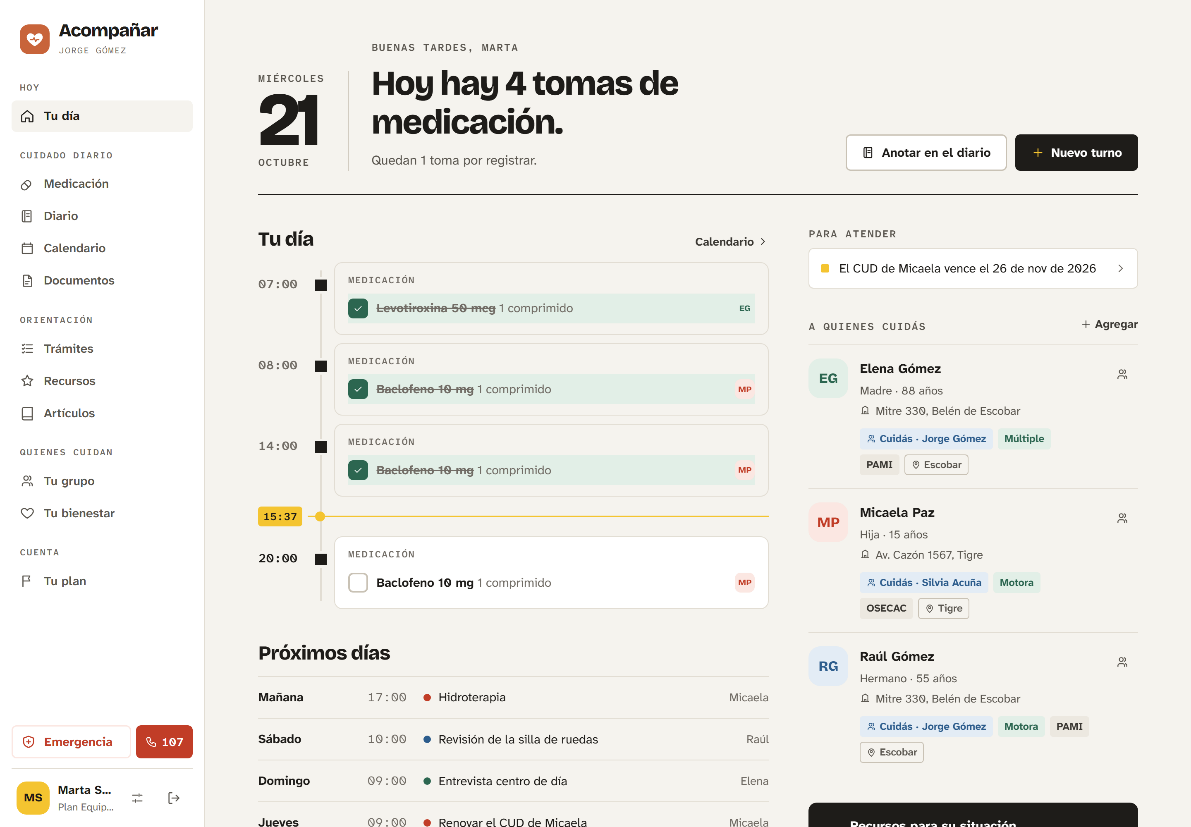
\includegraphics[width=\textwidth]{figuras/fig-4-1}
\caption{Tu día de una cuidadora contratada que atiende a personas de dos familias}\label{fig:fig-4-1}
\end{figure}

\begin{figure}[H]
\centering
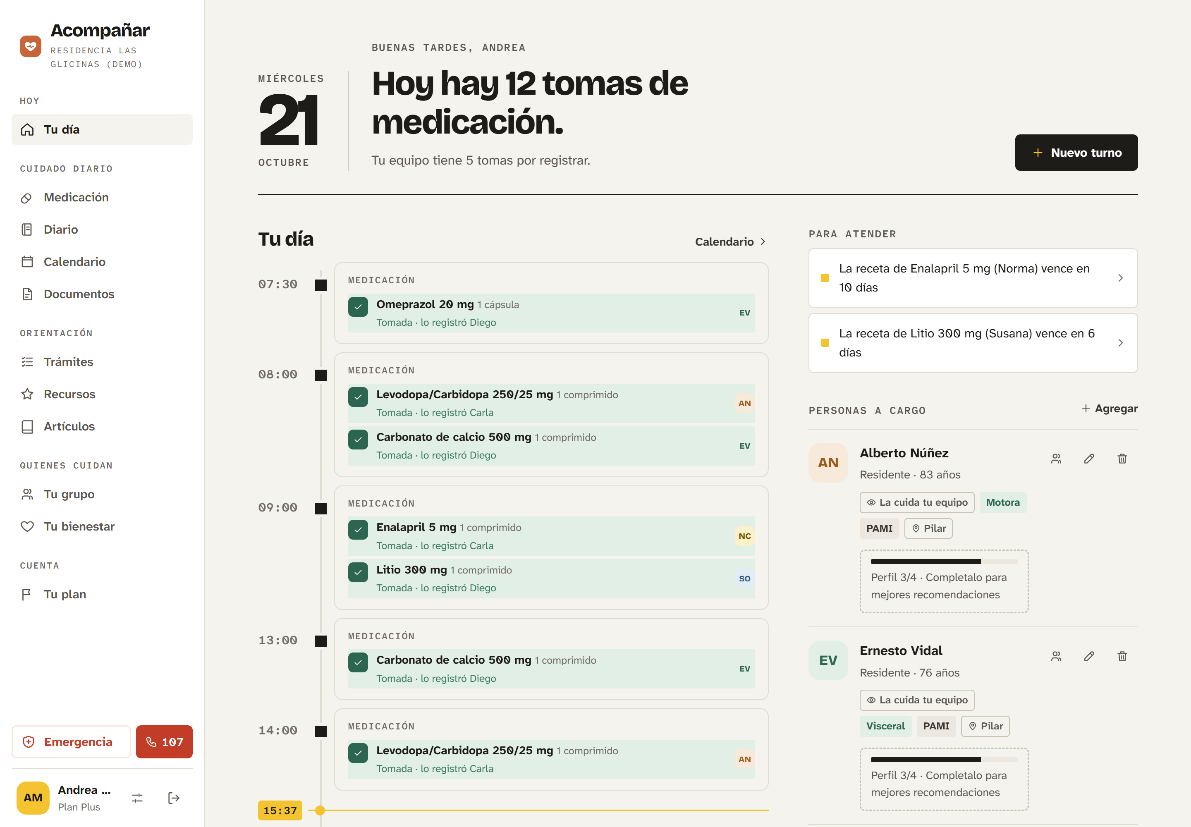
\includegraphics[width=\textwidth]{figuras/fig-4-2}
\caption{Tu día de la dueña de una residencia: el estado de cada toma y quién la registró}\label{fig:fig-4-2}
\end{figure}

\begin{figure}[H]
\centering
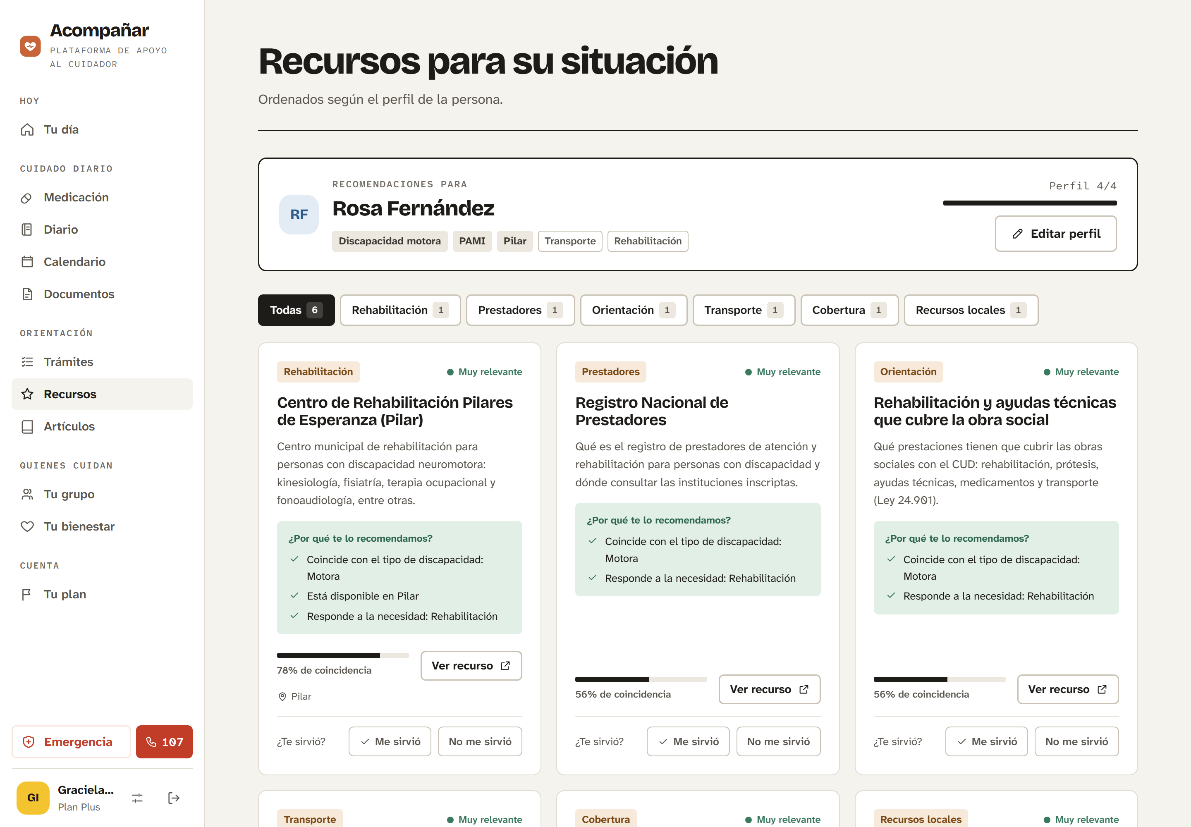
\includegraphics[width=\textwidth]{figuras/fig-4-3}
\caption{Recursos para la discapacidad de la persona, ordenados según su perfil, con su explicación y los botones de valoración}\label{fig:fig-4-3}
\end{figure}

\begin{figure}[H]
\centering
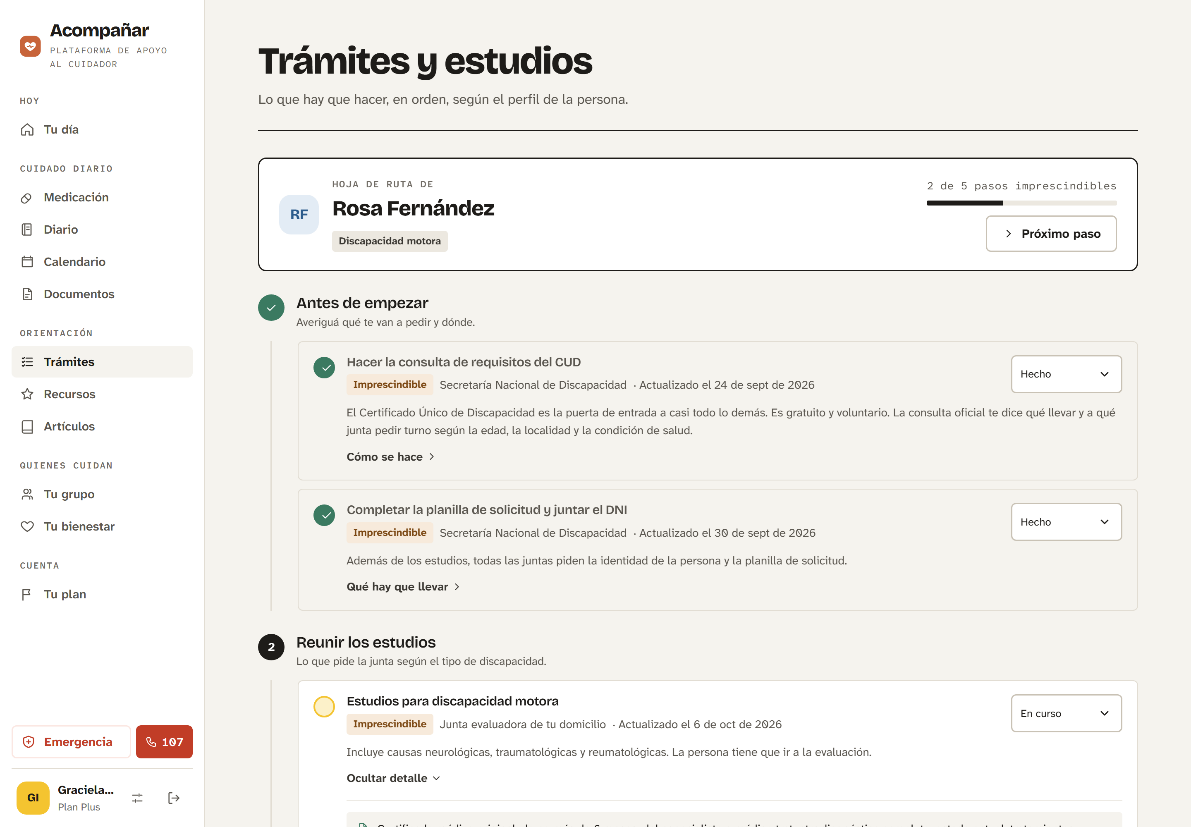
\includegraphics[width=\textwidth]{figuras/fig-4-4}
\caption{Hoja de ruta de trámites y estudios para el Certificado Único de Discapacidad}\label{fig:fig-4-4}
\end{figure}

\begin{figure}[H]
\centering
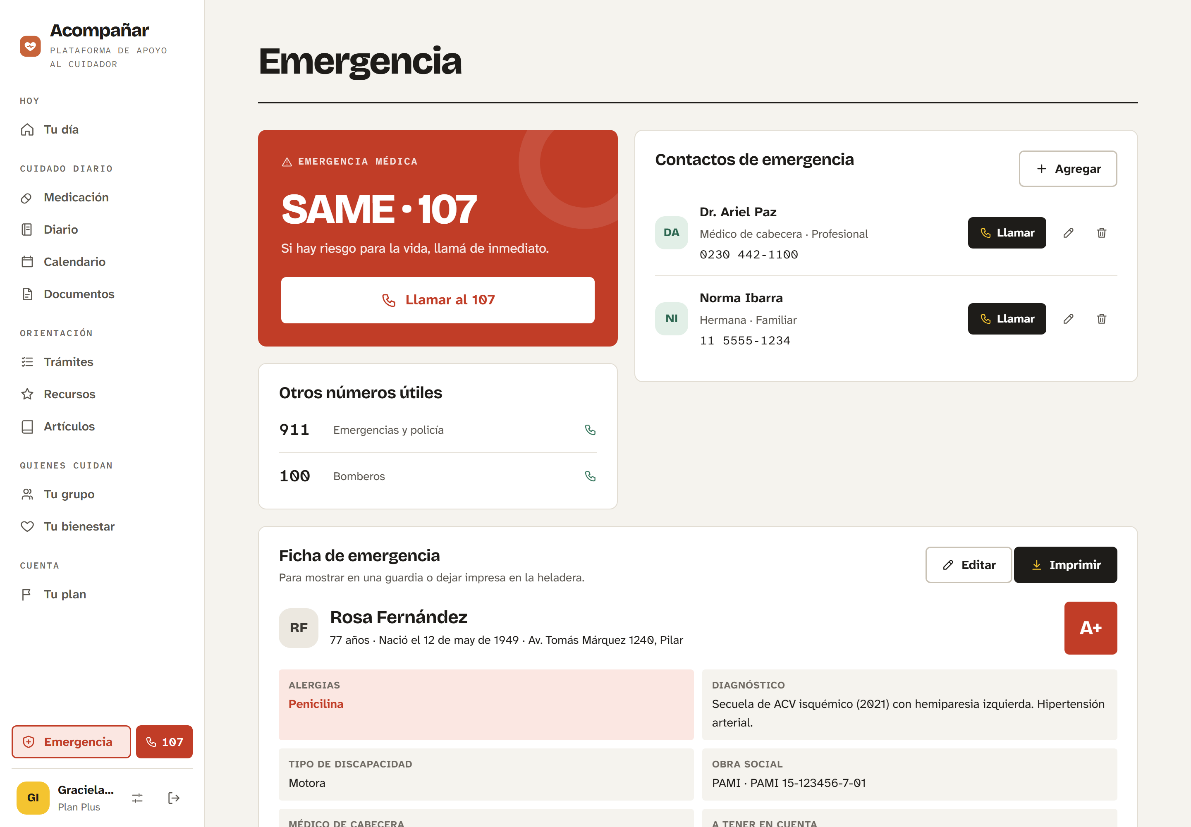
\includegraphics[width=\textwidth]{figuras/fig-4-5}
\caption{Módulo de emergencia con el acceso al 107, los contactos de la red de apoyo y la ficha}\label{fig:fig-4-5}
\end{figure}

\begin{figure}[H]
\centering
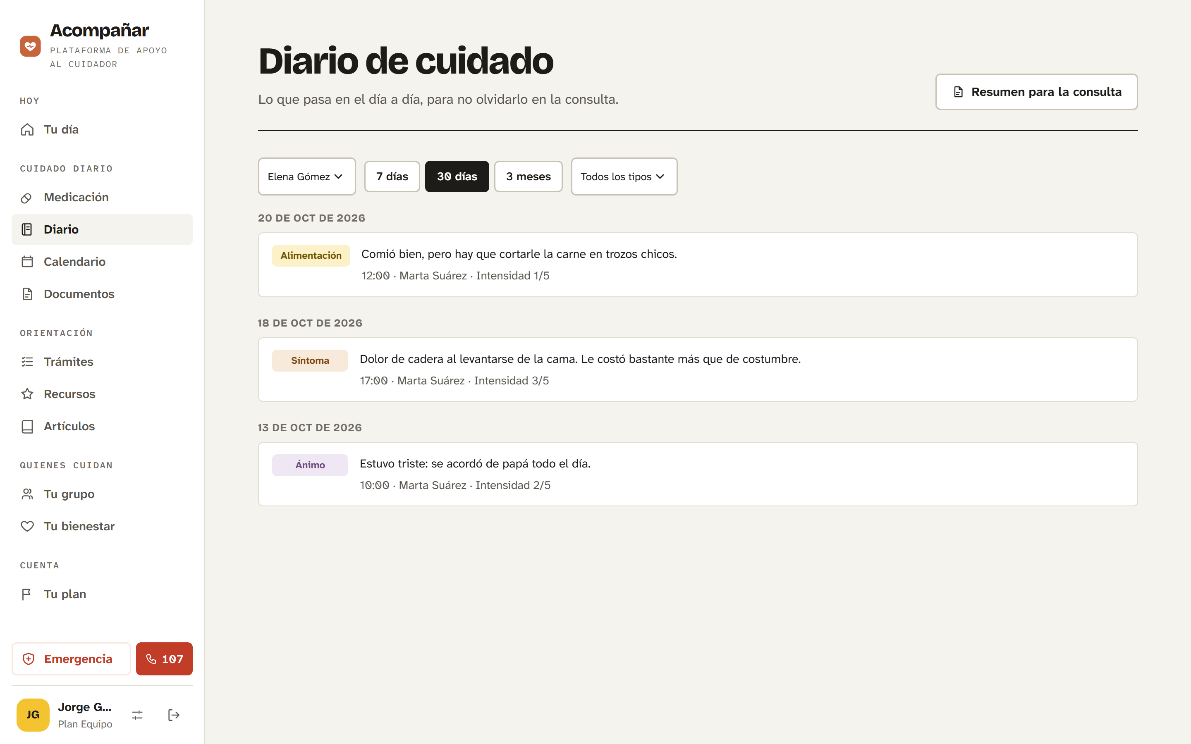
\includegraphics[width=\textwidth]{figuras/fig-4-6}
\caption{Diario visto por un familiar en modo observador. Los registros son de la cuidadora y no se pueden editar}\label{fig:fig-4-6}
\end{figure}

\begin{figure}[H]
\centering
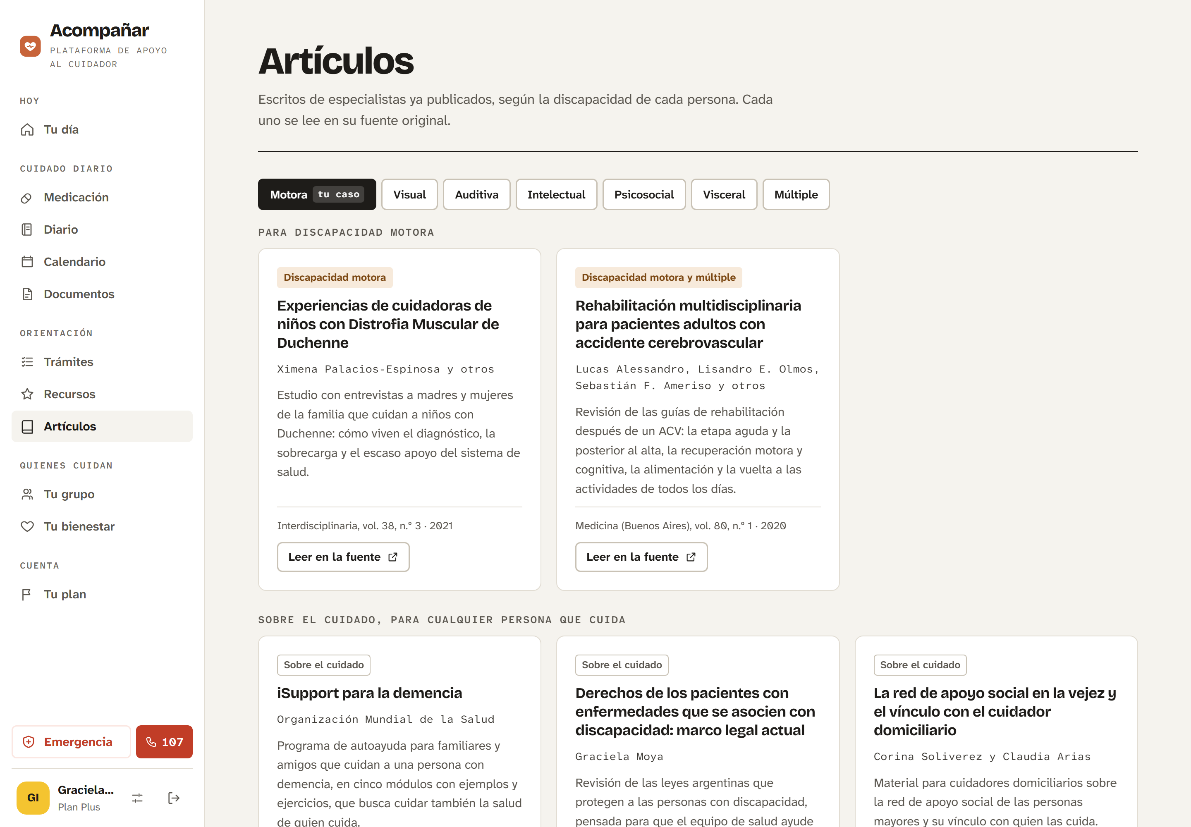
\includegraphics[width=\textwidth]{figuras/fig-4-7}
\caption{Artículos de especialistas para la discapacidad de la persona y, aparte, los generales sobre el cuidado}\label{fig:fig-4-7}
\end{figure}

\begin{figure}[H]
\centering
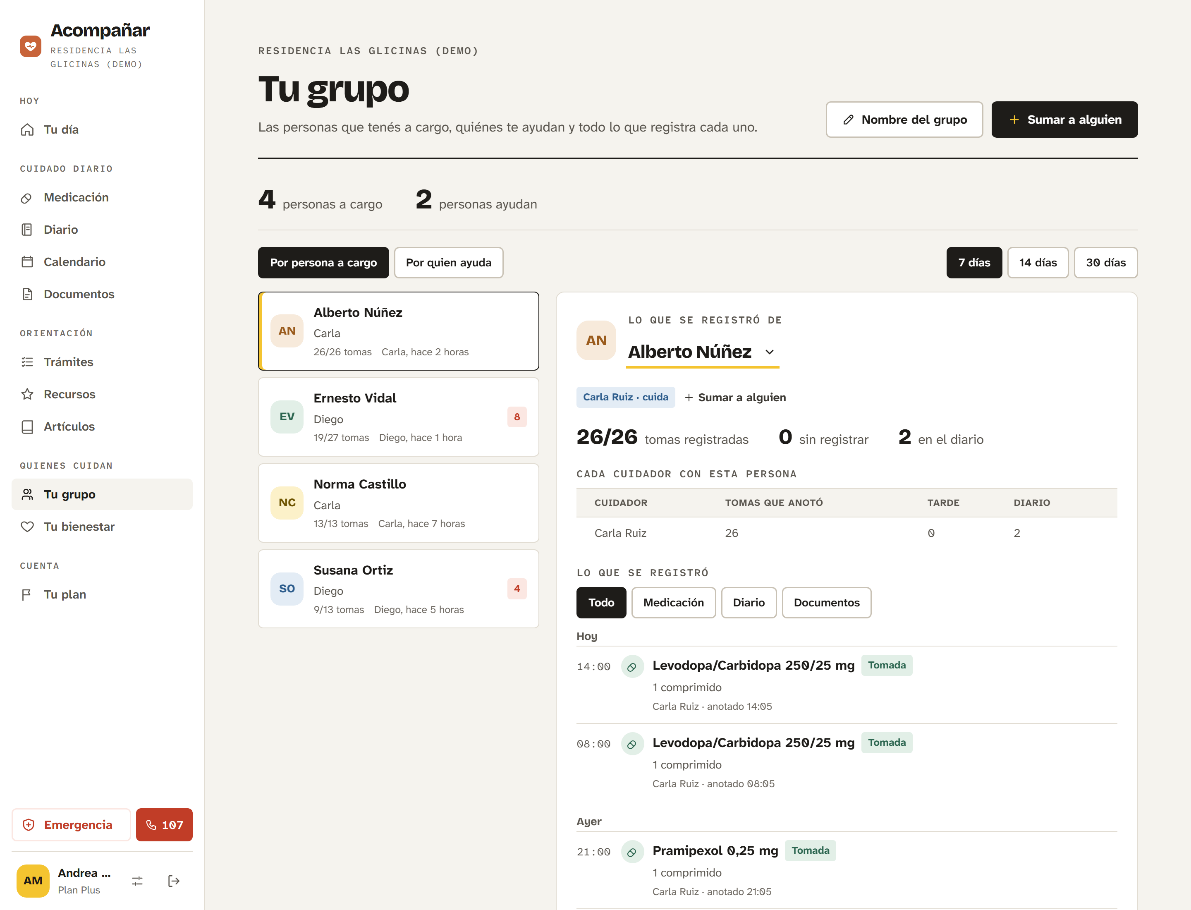
\includegraphics[width=\textwidth]{figuras/fig-4-8}
\caption{Tu grupo visto por la dueña de una residencia: cada residente, quién lo cuida y todo lo que se registró}\label{fig:fig-4-8}
\end{figure}

\begin{figure}[H]
\centering
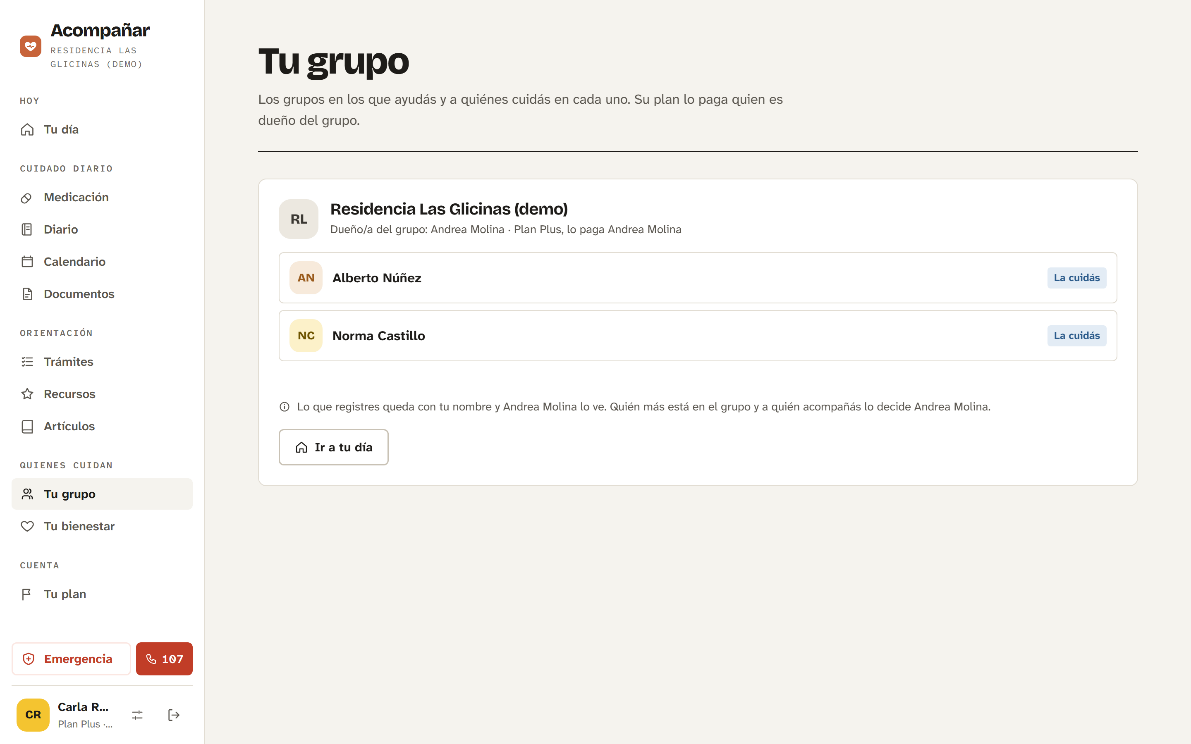
\includegraphics[width=\textwidth]{figuras/fig-4-9}
\caption{Tu grupo visto por una cuidadora: el grupo en el que ayuda, a quiénes cuida y que el plan lo paga la dueña}\label{fig:fig-4-9}
\end{figure}

\begin{figure}[H]
\centering
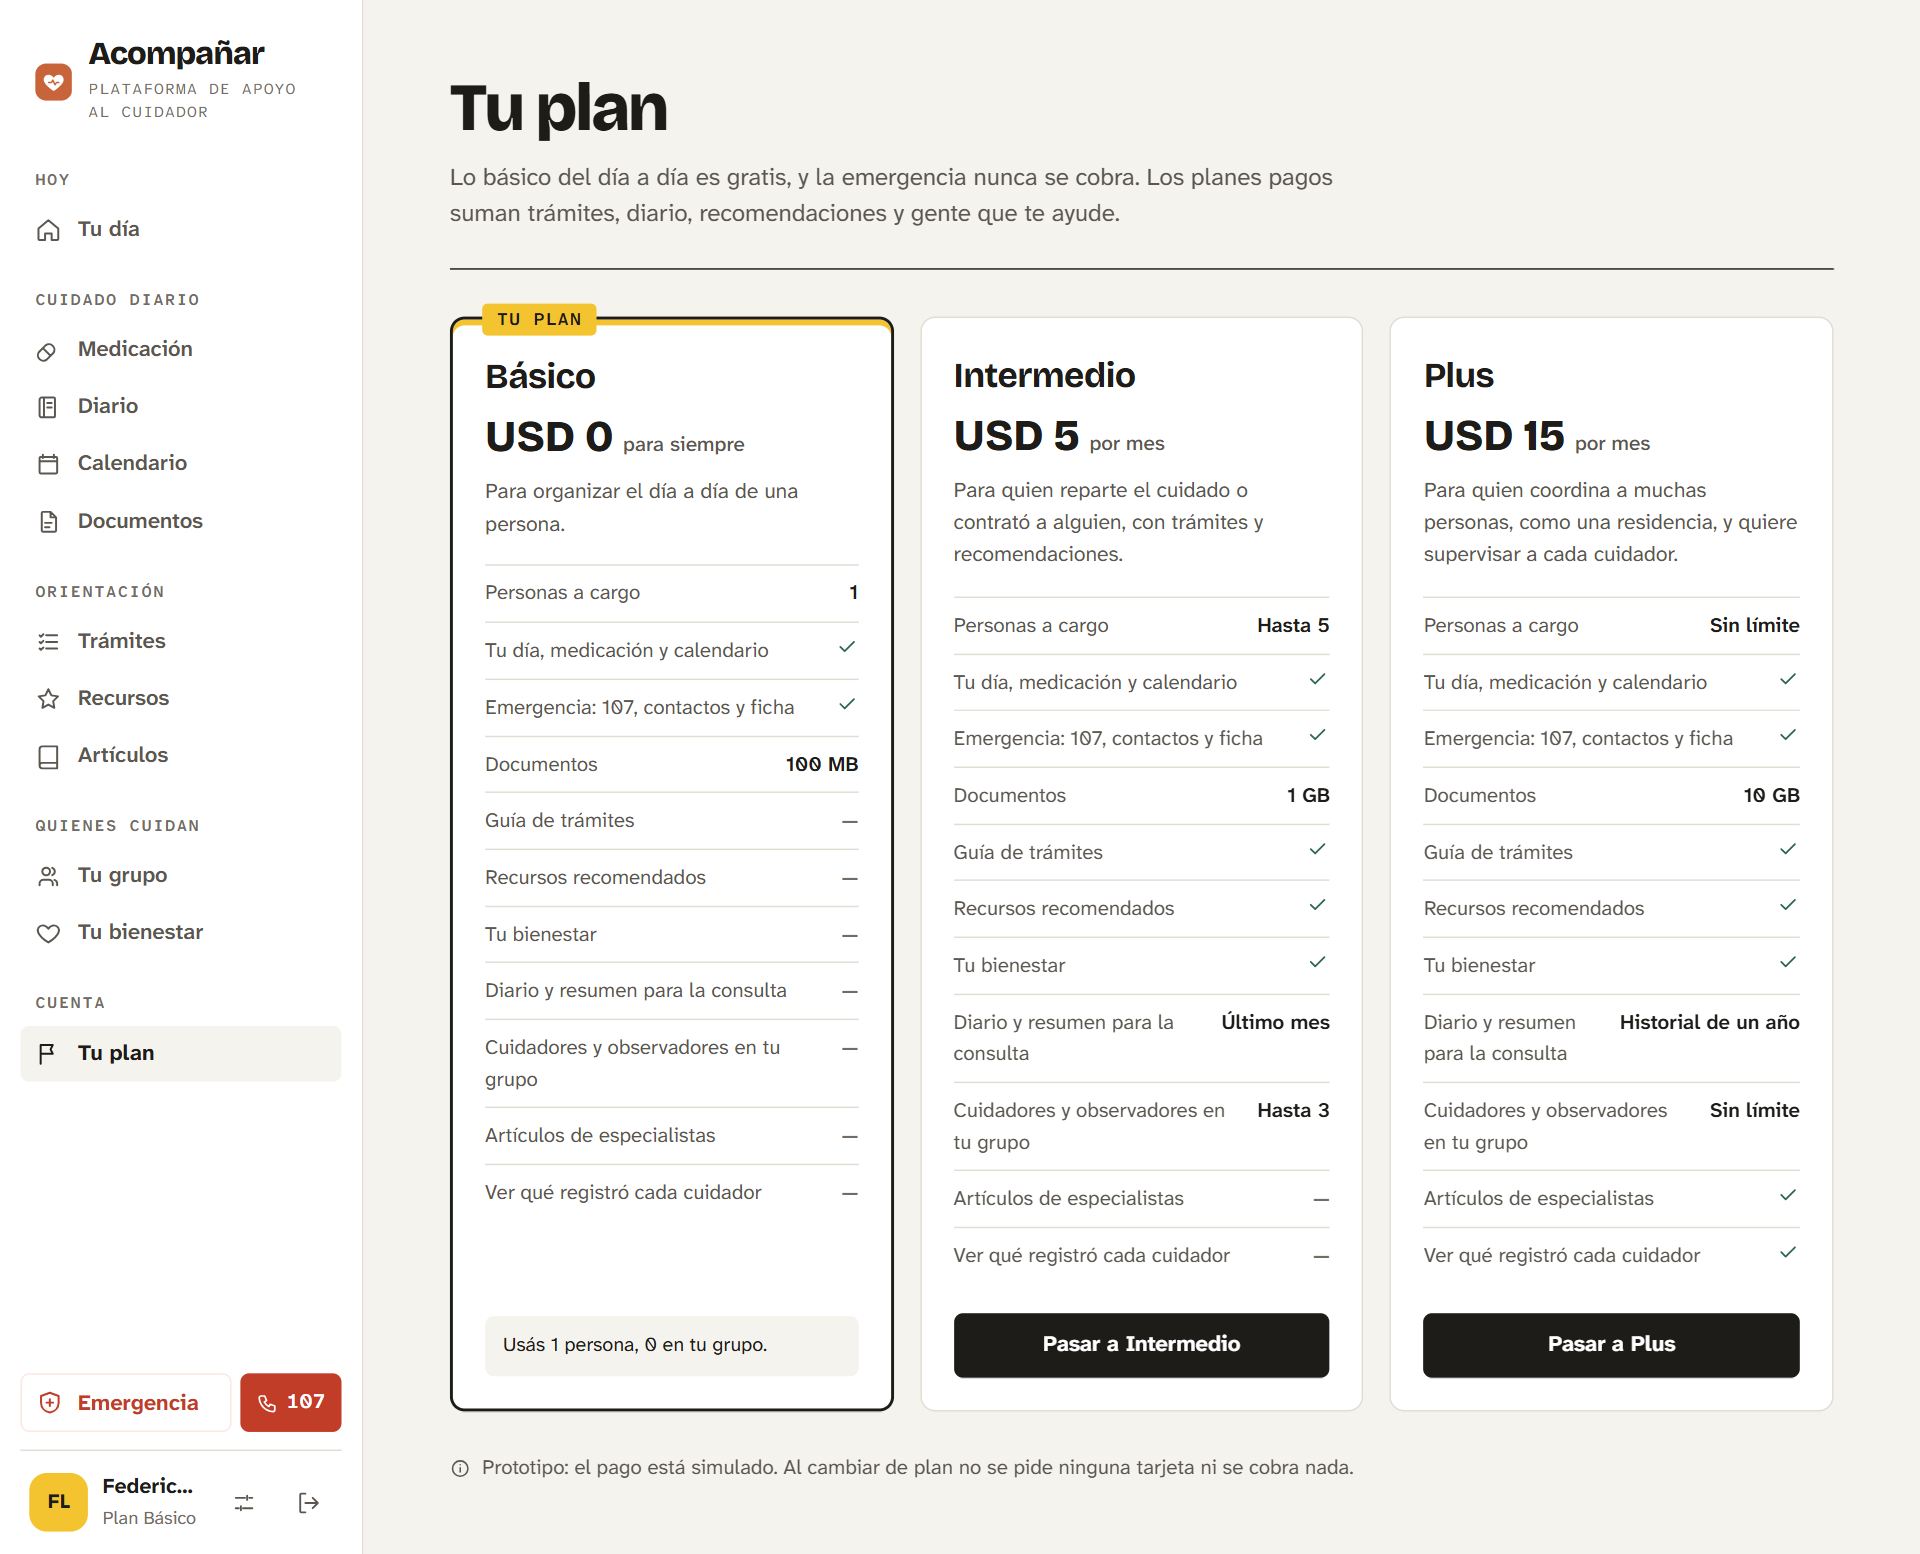
\includegraphics[width=\textwidth]{figuras/fig-4-10}
\caption{Planes Básico, Intermedio y Plus}\label{fig:fig-4-10}
\end{figure}

\begin{figure}[H]
\centering
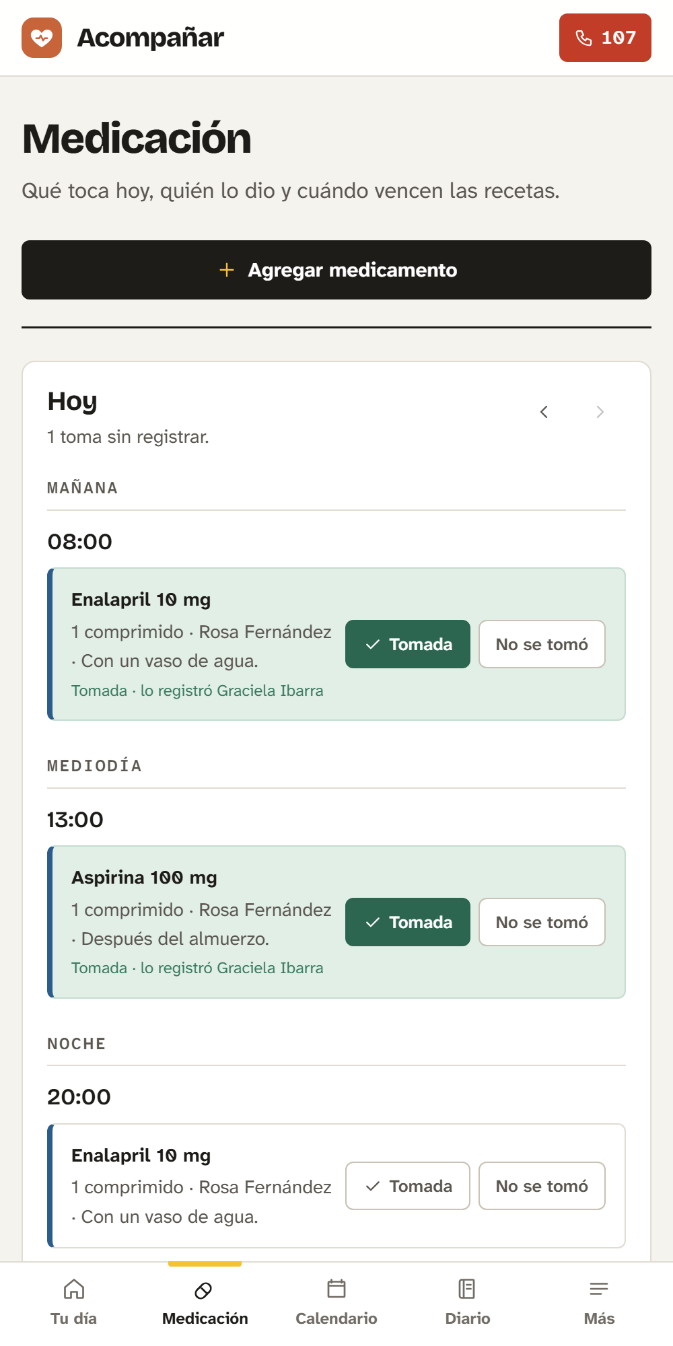
\includegraphics[width=0.35\textwidth]{figuras/fig-4-11}
\caption{Agenda de medicación en la versión para celular}\label{fig:fig-4-11}
\end{figure}

\section{Limitaciones actuales y próximos pasos}

\begin{itemize}
    \item Todavía no está publicada en la nube: Hoy la plataforma se ejecuta en un entorno local, con SQL Server Express y los datos de demostración. El próximo paso es publicarla en Azure, con la aplicación en Azure App Service y la base de datos en Azure SQL Database, para que se pueda usar desde cualquier navegador. Su comportamiento con muchos usuarios simultáneos todavía no se midió.
    \item El pago está simulado: El cambio de planes inmediato y no se cobra. Para cobrar hace falta integrar una pasarela de pagos.
    \item Faltan datos de uso reales: El componente colaborativo del recomendador está implementado, pero solo se probó con datos de demostración.
\end{itemize}

Los próximos pasos planificados son (1) validar el uso con cuidadores y con al menos una residencia, y (2) integrar una pasarela de pagos.

\section{Software}

La tabla~\ref{tab:c4-1} resume las tecnologías elegidas para la plataforma. Las versiones exactas de cada componente se detallan en el apéndice~\ref{apx:tecnicos}.

\begin{table}[H]
\centering
\caption{Tecnologías utilizadas}\label{tab:c4-1}
\small
\begin{tabularx}{\textwidth}{>{\raggedright\arraybackslash}X >{\raggedright\arraybackslash}X >{\raggedright\arraybackslash}X}
\toprule
\tb{Capa} & \tb{Tecnología elegida} & \tb{Motivo principal} \\
\midrule
Entorno de desarrollo & Visual Studio & IDE integrado con depurador y herramientas de perfilado ya conocidas. \\
Frontend web & React + Vite (JavaScript / JSX) & Interfaz reactiva y modular. Vite ofrece un entorno de desarrollo rápido sin la complejidad de un framework. \\
Backend / API & ASP.NET Core Web API (C\#, .NET 10) & Tipado fuerte, alto rendimiento y conocimiento previo, reduce errores en tiempo de compilación durante un desarrollo solitario. \\
Base de datos & SQL Server con Entity Framework Core & Motor relacional maduro y coherente con las entidades del dominio. Las migraciones versionan el esquema. \\
Documentación de API & Swagger & Documentación interactiva generada a partir del propio código de la API. \\
Autenticación & ASP.NET Core Identity y JWT & Registro, inicio de sesión, hash de contraseñas y roles integrados al framework. El token firmado identifica cada solicitud. \\
Pruebas & xUnit con SQLite en memoria & Pruebas automatizadas sobre una base relacional real que no afecta los datos del sistema. \\
Control de versiones & Git y GitHub (repositorio privado) & Historial de cambios y copia del código fuera del equipo de desarrollo. \\
\bottomrule
\end{tabularx}
\end{table}

\section{Frontend}

El frontend se construyó con React y Vite. Se eligió Vite en lugar de un framework con renderizado del lado del servidor, como Next.js, porque la plataforma no requiere ese tipo de optimización para su escala inicial, y Vite ofrece un servidor de desarrollo considerablemente más rápido con una configuración mucho más simple. La interfaz se organizó en componentes reutilizables, como las tarjetas de recomendación, la línea del día, las tarjetas de personas o los formularios.

En cuanto al acceso desde dispositivos móviles, se decidió no desarrollar una aplicación nativa separada, sino construir el frontend web como una interfaz responsive, capaz de adaptarse tanto a computadoras como a celulares desde un mismo proyecto. Esta decisión evita duplicar el desarrollo de una interfaz equivalente en una tecnología distinta. La interfaz se adapta además a lo que puede hacer cada usuario con cada persona, de modo que quien está en modo observador no ve los botones para registrar o editar.

\section{Backend y lógica de negocio}

Para la construcción de la API REST y el motor de recomendación se seleccionó ASP.NET Core Web API con C\#. La razón principal detrás de esta decisión fue el dominio previo que ya se tenía sobre estas tecnologías, lo que redujo significativamente la curva de aprendizaje y aceleró la puesta en marcha.

Trabajar con C\# ofrece una ventaja fundamental, su sistema de tipado fuerte. Esto significa que gran parte de los errores de código se detectan al momento de compilar y no cuando la aplicación ya se está ejecutando. En un escenario donde una sola persona asume todo el rol de desarrollo, pruebas y corrección de fallos, esta característica ayuda a mantener la estabilidad del sistema.

El control de acceso se concentró en un único servicio, que define qué puede hacer cada usuario con cada persona y que usan todos los controladores. Hay cuatro niveles. Ver, que tienen todos los integrantes del grupo, gestionar turnos, medicación, documentos, contactos y trámites, que tienen el dueño y los cuidadores, registrar tomas y diario, que tienen los cuidadores y el dueño solo si también cuida y administrar el perfil, la ficha y el grupo, que corresponde al dueño. Los límites de cada plan se controlan también en la API, tomando el plan del dueño de cada persona.

El motor de recomendación se mantuvo simple para no sobrecargar la arquitectura. No hizo falta incorporar librerías externas de inteligencia artificial o aprendizaje automático. Se programó como un servicio interno de la API, que solo considera los recursos del tipo de discapacidad de la persona, descarta los que piden otra obra social o localidad, aplica una función de puntaje ponderado y ajusta el orden según las valoraciones.

\section{Base de datos}

Se eligió SQL Server como motor de base de datos, en conjunto con Entity Framework Core como capa de acceso a datos. El dominio del problema es naturalmente relacional, por lo que un motor SQL resulta más adecuado que una base no relacional. Entity Framework Core, al trabajar con un enfoque code-first, permite definir el modelo de datos directamente en clases de C\# y generar el esquema de base de datos junto con sus migraciones de forma versionada.

El modelo de datos organiza la información a través de entidades como Usuario (con su plan y el nombre de su grupo), Persona asistida, Integrante del grupo, Turno, Medicamento, Toma, Entrada del diario, Documento, Contacto de emergencia, Avance de trámite, Recurso, Valoración de recurso, Artículo y Evaluación de esfuerzo.

Para asegurar que los datos se mantengan consistentes y bien relacionados, se aplican claves foráneas, borrado en cascada donde corresponde e índices únicos que evitan duplicados. La evolución del esquema se gestiona mediante las migraciones de Entity Framework Core, que al guardarse junto con el código permiten volver a una versión anterior ante cualquier eventualidad. Cuando el sistema se publique en Azure, las copias de seguridad quedarán a cargo de Azure SQL Database.

\section{Infraestructura y despliegue}

Por ahora el sistema se ejecuta en un entorno local, con SQL Server Express y los datos de demostración, y su publicación queda como próximo paso. Para esa etapa se eligió Microsoft Azure: la aplicación se publicará en Azure App Service y la base de datos en Azure SQL Database. Se eligió Azure por su integración directa con .NET y SQL Server, lo que permite desplegar sin cambiar el motor de base de datos ni el código de acceso a datos, y porque ofrece planes de bajo costo para una escala inicial. Las alternativas evaluadas fueron alojar la API en un servidor virtual propio, que exigía administrar el sistema operativo y las copias de seguridad, o pasar a una base de datos distinta de SQL Server, lo que obligaba a migrar el esquema.

Una vez publicado, la escalabilidad se resolverá con las opciones del proveedor. El plan de App Service puede aumentar su capacidad o la cantidad de instancias, y la base de datos puede pasar a un nivel de servicio superior sin cambiar la aplicación. Los costos de infraestructura previstos se presentan en el capítulo~\ref{cap:economica}.

El código se versiona en GitHub, y las migraciones de Entity Framework Core permiten reproducir el esquema de la base en cualquier entorno. El repositorio no incluye todavía un proceso automatizado de integración y despliegue continuos, por lo que las pruebas automatizadas deben ejecutarse de forma manual antes de publicar cada versión. La publicación en Azure, la automatización de ese proceso y la configuración de alertas de monitoreo sobre los registros y las métricas que ofrece Azure quedan como próximos pasos. El entorno local de desarrollo, con SQL Server Express y los datos de demostración, es el que se usa hoy para las pruebas y la demostración.

\section{Diseño y experiencia de usuario (UX/UI)}

Las decisiones de diseño aplican directamente los principios de diseño centrado en el usuario descriptos en el Capítulo 3, en particular la norma ISO 9241-210. Dado que la plataforma está pensada para cuidadores con niveles de familiaridad tecnológica muy dispares, se priorizó un lenguaje claro y directo, una navegación persistente (barra lateral en la versión de escritorio, barra inferior en la versión móvil) y la reducción del número de pasos necesarios para completar cualquier acción.

La identidad visual combina un fondo cálido, tipografía oscura y un solo color de acento, amarillo, que marca lo que requiere atención, como la hora actual o la sección activa. El rojo se reserva para la emergencia y cada persona asistida tiene un color propio, para reconocer a quién corresponde cada turno o toma. Se adoptó la tipografía Atkinson Hyperlegible, desarrollada por el Braille Institute \citep{braille2019} para personas con baja visión, y la plataforma permite agrandar el texto y activar un modo de alto contraste. El elemento de diseño más relevante sigue siendo la explicación ``¿Por qué te lo recomendamos?'' en cada recomendación, que responde a la necesidad de explicabilidad.

\section{Seguridad}

La autenticación de usuarios se implementó con ASP.NET Core Identity, el sistema de identidad integrado al propio framework, que gestiona el registro, el inicio de sesión, la recuperación de la contraseña y el hash seguro de contraseñas. Cada sesión se identifica mediante un token JWT firmado, emitido por la API tras un inicio de sesión exitoso y validado en cada solicitud posterior. Después de cinco intentos fallidos la cuenta se bloquea durante cinco minutos.

El control de accesos combina los roles de la cuenta (cuidador y administración) con el nivel de acceso de cada usuario sobre cada persona asistida, descripto en la sección de backend. Así, un cuidador contratado solo ve a las personas que tiene asignadas, un observador no puede modificar nada y nadie ve las personas del grupo de otro dueño. Los archivos que se suben se validan por su contenido real y no solo por su extensión.

El cifrado queda previsto para la publicación en Azure: allí los datos se guardarán cifrados en reposo mediante Transparent Data Encryption, que Azure SQL Database aplica de forma nativa, y viajarán cifrados con HTTPS/TLS. En el entorno local actual, que solo usa datos de demostración, no se aplica cifrado en reposo. Queda previsto reforzar la protección a nivel de base de datos mediante Row-Level Security de SQL Server. Dado que la plataforma maneja información sensible sobre la salud de terceros, el tratamiento de los datos se ajustará a lo previsto por la Ley 25.326 de Protección de Datos Personales.

